%%% LaTeX Template: Newsletter
%%%
%%% Source: http://www.howtotex.com/
%%% Feel free to distribute this template, but please keep the referal to HowToTeX.com.
%%% Date: September 2011


%%% ---------------
%%% PREAMBLE
%%% ---------------
\documentclass[10pt,a4paper]{article}

% Define geometry (without using the geometry package)
\setlength\topmargin{-48pt}
\setlength\headheight{0pt}
\setlength\headsep{25pt}
\setlength\marginparwidth{-20pt}
\setlength\textwidth{7.0in}
\setlength\textheight{9.5in}
\setlength\oddsidemargin{-30pt}
\setlength\evensidemargin{-30pt}

\frenchspacing						% better looking spacing

% Call packages we'll need
\usepackage[english]{babel}			% english
\usepackage{graphicx}				% images
\usepackage{amssymb,amsmath}		% math
\usepackage{multicol,caption}				% three-column layout
\usepackage{url}					% clickable links
\usepackage{marvosym}				% symbols
\usepackage{wrapfig}				% wrapping text around figures
\usepackage[T1]{fontenc}			% font encoding
\usepackage{charter} 				% Charter font for main content
\usepackage{blindtext}				% dummy text
\usepackage{datetime}				% custom date
	\newdateformat{mydate}{\monthname[\THEMONTH] \THEYEAR}
\usepackage[pdfpagemode=FullScreen,
			colorlinks=false]{hyperref}	% links and pdf behaviour
\usepackage{hyperref}



% Customize (header and) footer
\usepackage{fancyhdr}
\pagestyle{fancy}
\fancyhf{}
\lfoot{}
%\lfoot{	\footnotesize 
%		Newletter from HowToTeX.com \\
%		\Mundus\ \href{http://www.howtotex.com}{HowToTeX.com}	\quad
%		\Telefon\ 555-5555											\quad
%		\Letter\ \href{mailto:frits@howtotex.com}{frits@howtotex.com}
%	  }
\cfoot{}
\rfoot{\footnotesize ~\\ Page \thepage}
\renewcommand{\headrulewidth}{0.0pt}	% no bar on top of page
\renewcommand{\footrulewidth}{0.4pt}	% bar on bottom of page

%%% ---------------
%%% DEFINITIONS
%%% ---------------

% Define separators
\newcommand{\HorRule}[1]{\noindent\rule{\linewidth}{#1}} % Creating a horizontal rule
\newcommand{\SepRule}{\noindent							 % Creating a separator
						\begin{center}
							\rule{250pt}{1pt}
						\end{center}
						}						

% Define Title en News input
\newcommand{\JournalName}[1]{%
		\begin{center}	
			\Huge \usefont{T1}{augie}{m}{n}
			#1%
		\end{center}	
		\par \normalsize \normalfont}
		
\newcommand{\JournalIssue}[1]{%
		\hfill \textsc{\mydate \today, No #1}
		\par \normalsize \normalfont}

\newcommand{\NewsItem}[1]{%
		\usefont{T1}{augie}{m}{n} 	
		\large \bf #1 \vspace{4pt}
		\par \normalsize \normalfont}
		
\newcommand{\NewsAuthor}[1]{%
			\hfill by \textsc{#1} \vspace{4pt}
			\par \normalfont}		

\newcommand\sect[1]{%
  \section*{#1}%
  \addcontentsline{toc}{section}{#1}}

\newcommand\subsect[1]{%
  \subsection*{#1}%
  \addcontentsline{toc}{subsection}{#1}}


\newcommand{\HRule}{\rule{\linewidth}{0.5mm}}


\newenvironment{Figure}
  {\par\medskip\noindent\minipage{\linewidth}}
  {\endminipage\par\medskip}

%%% ---------------
%%% BEGIN DOCUMENT
%%% ---------------
\begin{document}



\begin{titlepage}

\begin{center}


% Upper part of the page
\includegraphics[width=0.5\textwidth]{pics/ecplogo.jpg}\\[1cm]    

\HRule \\[0.4cm]
{ \Huge \bfseries THE EXPLORER}\\[0.4cm]

\HRule \\[1.5cm]


\textsc{\LARGE January 2013}\\[9cm]

\textsc{\large The EXPLORER is the monthly newsletter of the Explorers Club Of Pittsburgh,Inc., a non-profit organization devoted to research, adventure and education in outdoor and wilderness recreation and conservation}\\[0.5cm]


% Title

% Author and supervisor
%\begin{minipage}{0.4\textwidth}
%\begin{flushleft} \large
%\emph{Author:}\\
%John \textsc{Smith}
%\end{flushleft}
%\end{minipage}
%\begin{minipage}{0.4\textwidth}
%\begin{flushright} \large
%\emph{Supervisor:} \\
%Dr.~Mark \textsc{Brown}
%\end{flushright}
%\end{minipage}

\vfill

% Bottom of the page
%{\large \today}

\end{center}

\end{titlepage}


% Title	
% -----
\JournalIssue{1}
\JournalName{The EXPLORER}
\noindent\HorRule{3pt} \\[-0.75\baselineskip]
\HorRule{1pt}
% -----

\tableofcontents

\clearpage


% Front article
% -----
\vspace{0.5cm}
	\SepRule
\vspace{0.5cm}



\begin{center}
\begin{minipage}[h]{0.8\linewidth}
	\begin{wrapfigure}{l}{0.41\textwidth}
		\includegraphics[width=0.6\linewidth]{pics/me.jpg}
		\\% this spacer is needed to make the text on the right fit OK
	\end{wrapfigure}
	
	\NewsItem{Message from the editor}
	\emph{Greetings, ECP!} Let me wish you a very happy new 2013. Welcome to the new edition of the club newsletter. The newsletter has undergone some formatting and editing changes. It has moved from microsoft word publishing system to \LaTeX. This means prettier newsletters ! Also the way in which the content was organized has changed. The trip reports have been brought to the front. The content of the magazines still remains the same, only some formatting changes. The magazine is also version controlled and can be accessed from \url{https://github.com/smoitra87/magecp} 	
\\
\\
	In this edition of the newsletter you will find trip reports of Alana Gilman hiking the Grand Canyon, John Zolko and Sam Taggart backcountry skiing in at St Marci, Utah hiking trip by Bill Baxter and part 4 of the alumni Nanga Parbat journal. The ECP has awarded some new life member cards. The activities pursued by the club and the officers in charge. Club business such as minutes from the club general meeting, BOG meeting, the treasurer report, the librarian report and the mountaineering school report. We also include an environmental article by Ginette Vinski. New members applying to be members of the club are listed. Finally, we include contact information of officers and an enrollment form in the end. 
\\
\\
-- Subhodeep Moitra (Deep)

\vspace{0.5cm}

	Again as a reminder, you are invited to attend the club general meeting and BOG member are requested to attend the BOG meeting. The meeting times for this month are :
	
\vspace{1cm}

\begin{multicols}{2}
\Large
JANUARY GENERAL MEETING\\
Thursday, January 10, 7:30PM\\
The Union Project (Highland Park Area)\\
841 North Negley Avenue

JANUARY BOG MEETING\\
Thursday, January 17th 7:30PM\\
at Bill Baxter's Home



\normalsize
\end{multicols}
	
\end{minipage}
\end{center}
% -----



\pagebreak
\clearpage


% Other news (1)
% -----
\vspace{0.5cm}
	\SepRule
\vspace{0.5cm}
\begin{multicols}{2}

\sect{Trip and Event Reports}

\subsect{Grand Canyon - Alana Gilman}
\textbf{Park Name:} Grand Canyon National Park, South Rim, Arizona\\
\textbf{Hikers:} Alana Gilman \& Rahul Shah\\
\textbf{Trail Name:} Rim Trail/Hermit's Rest Trail/Tonto Trail West/Bright Angel Trail\\
\textbf{Date In:} December 27, 2012\\
\textbf{Date Out:} December 29, 2012\\
\textbf{Total Distance}: 32.5 miles\\

\begin{Figure}
 \centering
 \includegraphics[width=0.95\linewidth]{pics/day0_1.jpg}
 \captionof{figure}{Day 0: Looking over the rim at the adventure ahead}
\end{Figure}

	
\textbf{Original Itinerary: }\\
	\textbf{Day 0:} Arrive at park. Camp at Mather Campground on rim.\\
\textbf{	Day 1} (12 miles): Hitchhike 8 miles along rim trail/road to Hermit's Rest Trailhead (free shuttle does not operate Dec-Feb). Hike 7.0 miles to Tonto Trail West junction and 5 miles to BL5 campground (Salt Creek).\\
\textbf{	Day 2} (13.5 miles): Hike 8 miles along Tonto Trail West to Indian Gardens. Hike 5.5 miles to Bright Angel Campground on Bright Angel Trail. Dinner reservations at Phantom Ranch restaurant.
\textbf{	Day 3} (8.5 miles): Breakfast at Phantom Ranch restaurant. Hike 8.5 miles on South Kaibab Trail to rim.

\begin{Figure}
 \centering
 \includegraphics[width=0.95\linewidth]{pics/day0_2.jpg}
 \captionof{figure}{Day 0: Camping at the rim }
\end{Figure}


\textbf{Actual Itinerary:}\\
\textbf{	Day 0:} Arrive at park. Camp at Mather Campground on rim.\\
\textbf{	Day 1} (17.3 miles): Hike 8.0 miles along rim trail to Hermit's Rest Trailhead. Hike 7.0 miles to Tonto Trail West junction and 2.3 miles to BL7 campground (Monument Creek).\\
\textbf{	Day 2} (10.7 miles): Hike 10.7 miles along Tonto Trail West to Indian Gardens Campground.\\
\textbf{	Day 3} (4.5 miles): Hike 4.5 miles along Bright Angel Trail to rim.

\begin{Figure}
 \centering
 \includegraphics[width=0.95\linewidth]{pics/day1_1.jpg}
 \captionof{figure}{Day 1: A frosty sunrise at the rim }
\end{Figure}

Our first backpacking trip of the Grand Canyon did not go according to plan, starting with Day 0 when we arrived at the park to find that the road to Hermit's Rest Trailhead was closed to all traffic due to winter weather conditions. We decided to modify our itinerary to include the 8 mile hike along the rim trail to arrive at the trailhead. At the backcountry office, we were able to change our Day 1 campsite to BL7 (Monument Creek), 2.7 miles closer than BL5 to account for the extra mileage along the rim, making our Day 1 total distance 17.3 miles rather than 12 miles and Day 2 total distance 16.2 miles rather than 13.5 and Day 3 unchanged. \\

\begin{Figure}
 \centering
 \includegraphics[width=0.95\linewidth]{pics/day1_2.jpg}
 \captionof{figure}{Day 1: Morning view from hike along the rim to Hermit's Rest Trailhead }
\end{Figure}

On the morning of Day 1, we left Mather campground at 5:20am in a snowstorm and arrived at Hermit's Rest Trailhead at 10am (30 minute stop at Bright Angel Lodge to fill water). We were unsure of whether water would be available at the trailhead due to the closed road and carried a full 7.5 liters to the BL7 campsite. At the trailhead after 8 miles along the rim, we felt strong and energized after stopping to make breakfast and chat with a ranger who was delivering water. At 11am, we began the descent into the canyon along Hermit's Rest Trail. The trail conditions were snowy with some ice, but still passable without crampons. We did not see any other hikers throughout the day. Just about the time we were beginning to feel tired and the distance was wearing on us, we came upon a landmark section of the trail called “Cathedral Stairs”. It seems that a mountaineering school student can't escape the stairs even in Arizona! 


By the time we arrived at the Tonto Trail West junction, we had 2.3 miles left and were very sore and tired. It was 4pm and we hoped to arrive at camp before dark (sunset was around 5:30pm). We raced through the last section as quickly as possible and arrived at BL7 (Monument Creek) just in the nick of time to filter water from the creek and set up camp. There was one other party of two at the campsite.

\begin{Figure}
 \centering
 \includegraphics[width=0.95\linewidth]{pics/day1_3.jpg}
 \captionof{figure}{Day 1: Snow \& ice for the descent along Hermit's Rest Trail}
\end{Figure}

Day 2 is when the real drama of the trip began. We woke up at 3:30 to depart before sunrise to allow plenty of time for the long hike ahead and the anticipated soreness from the day before. Upon leaving camp around 5:30am, we walked 100 yards to the creek bed, where two cairns marked the way to the campsite coming from the East. However, there was no indication of the direction of the trail heading West. 

\begin{Figure}
 \centering
 \includegraphics[width=0.95\linewidth]{pics/day1_4.jpg}
 \captionof{figure}{Day 1: Hermit's Rest Trail. The scale of the canyon is truly incredible}
\end{Figure}


The map purchased in the giftshop on the rim was of such a small scale, that details like this one were impossible to discern. We tried to read contour lines and were certain the trail bent to the left around a large butte and to the right of the “monument” of Monument Creek. In the dark, it was too difficult to discern trail from river wash and after about 15 minutes, we decided to head back to the campsite to wait until sunrise at 7:30am to make another attempt. We killed time cooking breakfast and waiting for the sun (it was pitch black because all moonlight was blocked by the tall canyon walls). When we took off for the second time, we again headed to the left to find the trail. We scrambled around on rocks and scree, looking around corners, sometimes dropping our packs to scout and other times convincing ourselves that a few feet of dirt or lack of vegetation must be the trail, only to find another dead-end. Eventually, we found ourselves out on the side of a formation, no trail in sight, scrambling around near the ledge of a 1,000+ ft dropoff when I tripped and hit the ground hard.

\begin{Figure}
 \centering
 \includegraphics[width=0.95\linewidth]{pics/day2_1.jpg}
  \captionof{figure}{Day 2: The Tonto Trail West}
\end{Figure}

 That was the low point when we realized that we were far from our goal and needed to give up this futile search. This highly traveled trail couldn't possibly involve this kind of scrambling and no markings. We hoped that the other campers were still at the campsite to give directions since they had arrived from the East the night before. We found them eating breakfast and they led us up the creek bed to the right to a small, barely-marked trail entrance at least 200 yards away. We were dumbfounded how anyone could be expected to find the trail without any indication of direction when traveling from the West, exasperated that 

we spent two hours searching needlessly (and dangerously) to the left, and frustrated that we were now four hours behind our desired departure time, leaving at 9:30am. But we left all of that behind at the campsite and took off with renewed energy, calculating that with an average pace of 1.8 mph (a very manageable speed despite our sore legs and heavy packs) we could still make it to the Bright Angel Campground by 5pm for our dinner at Phantom Ranch restaurant. 

\begin{Figure}
 \centering
 \includegraphics[width=0.95\linewidth]{pics/day2_2.jpg}
  \captionof{figure}{Day 2: The inner canyon, Tonto Trail West}
\end{Figure}

But those delicious steaks were not to be our fate that night. Just when we were hitting our stride, Rahul began to slow down, complaining of knee pain. It seemed that the weight, excessive mileage from the previous day, and scrambling around left him with an overuse injury. Even though the trail for the day was relatively flat, his knee hurt with any kind of flexion. We wrapped it in an ace bandage and gave him some painkillers, but pretty soon our pace was down to a crawl. Suddenly, our priorities changed from making it to dinner to making it out of the canyon. We were 20 miles in and 20 miles out, without a ranger station in reach for at least 10 miles. The 13 miles left for that day would be impossible, as would the 9 mile hike out on South Kaibab the next day. We shifted ~15lbs from his pack to mine, and moved at a slow but steady pace. We set our sites on the Indian Gardens campground, only 10.7 miles from our starting point that day and, more importantly, 4.5 miles from the rim. This modified route would keep us from descending another 1,500 feet into the canyon and thus, having to ascend that same amount the next day. We struggled to arrive at Indian Gardens before sunset and limped in around 5:20pm.  My feet were killing me from the ~45 lb pack and Rahul's knee was in bad shape. Normally, this is a packed campground and a permit is required year-round, but the snowstorm and cold temperatures worked in our favor and there was a site available, which we used despite our lack of permit. As we rationed our remaining food and ate cashews for dinner we dreamt of the steak and cornbread we were missing out on at the bottom. 

In the morning, we continued with the slow and steady plan. I again carried the majority of the weight as we lumbered out of the canyon, one step at a time. We made it to the top and celebrated our victory. The trip didn't look anything like we had planned, but we had a blast and both made it out relatively unscathed. Rahul's knee is healing well and no permanent damage was done. We're already planning our return trip to explore the Tonto Trail East with a longer itinerary but more time for rest and shorter mileages each day. Hopefully this time those steaks won't elude us. They should be twice as good on the second try! 

\begin{Figure}
 \centering
 \includegraphics[width=0.95\linewidth]{pics/day2_3.jpg}
 \captionof{figure}{Day 3: Goodbye to the canyon, Bright Angel Trail}
\end{Figure}

\textbf{Food log: }\\
2 breakfasts: oatmeal, coffee, honey stinger waffles\\
	3 trail day lunches: salami, parmesan cheese, beef jerky, clif bars, trail mix, candy, sweet \& salty bars, dried fruit\\
	2 dinners: Mountain House dehydrated meals
\\
\\
\textbf{Water log:} 7.5 liter total capacity\\
	Day 1: Bright Angel Lodge water fountain, Monument Creek (filter in field)\\
	Day 2: Monument Creek (filter in field), Indian Gardens tap\\
	Day 3: Indian Gardens tap
\\
\\
\textbf{Weather:}\\
	Day 0: High 33, Low 9 with light snow, 2” accumulation\\
	Day 1: High 40, Low 20 with snow down to 4 miles below rim\\
	Day 2: High 45, Low 15 clear sky, no precipitation/wind\\
	Day 3: High 30, Low 15 clear sky, no precipitation/wind
\\
\\
\textbf{Gear:} ~38lb pack weight with water\\
	2 person/3 season tent w/ fly \\
0o sleeping bags with reactor extreme +25O liners\\
	Sleeping pads insulated \& inflatable\\
	Sit pad inflatable \\
Wire mesh animal proof food storage bag\\
	Jetboil stove with 110g isobutane/propane fuel canister\\
	Headlamps \\
Hiking poles\\
	Crampons (did not use, would have preferred yaktracks or microspikes)\\
	Scarpa Goretex Mountaineering boots\\
	Down booties as camp shoes (best gear of the trip!)\\
	Belay jackets (left at rim lodge and didn't need)\\
	Rain jacket/pants \& pack covers	\\
	Nanopuff down or primaloft\\
	Base layer long john pants \& shirt\\
	Liner gloves, beanie hats/earmuffs\\
	Nalgenes w/o insulated sleeves\\
	Camelback bladders (didn't freeze at night)\\
	Sunglasses/sunscreen (did not use)
\\
\\	
\textbf{Permit Information: }\\
Day 0: Mather campground at rim is first come/first serve in person with limited campsites accessible during winter months. 99\% of campsites were unoccupied. $15/campsite ($8 with annual national park pass

Days 1 and 2: Backcountry camping permits obtained through the Backcountry office via snail mail. Applied in October and did not receive first choice itinerary for campsite BL6 on 12/27. Permit approval received by mail in early December with required waiver of experience and risks for aggressive itinerary for hikes of >10 miles/day. Limited capacity at small campgrounds. Size of camps: 1 space at BL5, 1 space at BL6, and 3 spaces at BL7. Bright Angel campground and Indian Gardens Campgrounds are much bigger but also more popular. 

Permit was originally for BL5 (Salt Creek) on 12/27 and CBG (Bright Angel) on 12/28. Total cost: \$30 (\$10 for permit application and \$5/person/night). Permit adjusted to BL7 (Monument Creek) for 12/27 at Backcountry office on day 0 due to weather and road closure to Hermit's Rest Trailhead.
\\
\\
\textbf{Difficulty: }\\
\textbf{Rim Trail:} easy, flat, paved in some areas and wide dirt path in others, frequent distance markers, close to road, snow-covered\\
\textbf{	Hermit's Rest Trail:} moderately difficult, uneven steps, rocky terrain throughout, close to ledge, steep descents, long traverses, easy to navigate, clear trail, no water source, shade throughout day, light snow/ice cover with rocks down to 4 miles from rim\\
\textbf{	Tonto Trail West:} difficult, flat trail, unmarked junctions, clear but narrow dirt path, close to ledge, poorly defined entrance/exit from campsites, misplaced cairns near confusing junctions/creeks/landmarks, no snow/ice\\
\textbf{	Bright Angel Trail:} moderate, well-defined/maintained wide trail, easy to navigate, high traffic, minimal ledge exposure with rock border, multiple rest houses w/ emergency phones, steep ascent (3,000ft in 4.5 miles), snow/ice beginning at 3 mile house to rim with sand treatment for traction

	Most difficult parts of trip were routefinding at campsite junctions along Tonto Trail West and total distance on Day 1. Water source reliability was not as described by backcountry office at multiple campsites within canyon. Dry creeks.

\pagebreak

\subsect{Hiking in Colorado \& Utah - Baxter/George}

\small
{\it \dots At the end of the "Ledges", the "Trough" begins. This was an area of concern, since several climbers had told us there was snow and ice requiring going off route. As I came around the corner I was surprised, however, to see the amount of waterfall ice on one side. We had no crampons or ice axes but as it turned out they would not have made a difference \dots}
\normalsize

\begin{Figure}
 \centering
 \includegraphics[width=0.95\linewidth]{pics/tom_bill.jpg}
 \captionof{figure}{Bill Baxter and Tom George from a Colorado \& Utah hiking trip}
\end{Figure}

This an excerpt from a detailed trip report by Tom George. The full trip report can be found at \url{http://www.tomcentral.com/colutahweb/index.php}


\subsect{Backcountry Ski Trip - John Zolko, Sam Taggart}
We left at 6 am and did not get back out of the woods till 9:30 at night. We had equipment problems with our rental skis, boots would not clip into bindings, we broke 3 ski poles, got off trail, made it to withi .5 miles of the top. 8 miles up and 8 miles back and our last sign said .6 miles to the ridge and 1.2 miles to the summit. We made it to the edge of the ridge and turned around because it was late 2:30 and it was cold 5 degrees and wind blowing 20 to 30 mph.We came back with head lamps and ended up carrying skis out the last few miles.

A learning experience which included blisters on our feet, taking vicaden, no mole skin with us bridge on the dam was washed out, knee deep snow, rebar like branches on the bushwhacking we did when we got off trail.  Wiping out on the 18" wide down hill trail- had to ski down the trail we walked up.We were being passed by people on snow shoes. Wow ! My legs are still sore and i am still taking ibuprofen.

\subsect{Nanga Parbat - Andy Colucci's Journal - Chapter 4}
\textit{Historian's Note:  Andrew Colucci's hand-written journal of the Nanga Parbat Expedition - June 18 to August 19, 1977 - is one of the treasures in the ECP Archives.  Your historian has transcribed them into a typed computer file to supplement the precious original copy.  He submits it as a serial for publication in The Explorer.  Some spelling and punctuation corrections have been made in digitizing the journal; Others have been left as Andy entered them}.

\textit{What  follows is the fourth and final serial chapter of the Expedition Journal.
In previous chapters we read of the trip to Base Camp and Camp 1, and the difficult climb to Camp 2 at 19,600 ft.  We read of the health difficulties (dysentery, bloody feet, fatigue, and more) and the terrain difficulties and dangers.
}

\begin{Figure}
 \centering
 \includegraphics[width=0.95\linewidth]{pics/nanga_1.jpg}
\end{Figure}

 ( icy rocks and constant rock fall). In the last previous chapter we read how, day before this chapter begins, expedition leader George Bogel and his partner Bob Broughton were killed when a huge rock demolished the tent in which they were camped in a supply depot between camps 1 and 2.
\\
\\
\textit{Aug 1 - Mon.}
Hank came back in the middle of the night.  Everyone else bivied.  Peter, Dan got to Camp 2 in real bad shape.  They got there about 9PM.  Bruce said he had to feed Peter; that's how bad he was.  He started ranting and raging when he heard about George and Bob.  Bob, Hank, and I got up at 5AM and started up.  We found George's body around 7AM. About 900 feet up from Camp. He was killed instantly; he was broken up pretty good.

Ellery broke his ankle around 4AM traversing over to the Depot Rock.  Equipment was strewn all over the glacier.  Bruce and Nelson came down.  Peter and Dan stayed at Camp 2.  Bruce said a slab of rock 100' high came off a cliff about 150' from the Depot, and went right over the tent.  A lot of equipment is still up there.  We couldn't find Bob's body.  

Ellery has a severely broken ankle and will be carried down to Base tomorrow.  So will George.  Hank, Nelson, Rick, Jay, Bruce, and I dragged George's body down.  Will go up tomorrow for the rest of the equipment.  Jay went to Base to get things straightened out on the radio.  The L.O. Called out: 2 unidentified climbers killed.  That has to be straightened out and the names given out.

Bob I didn't know that well.  He was about 43.  George I was real close to; he will be missed sadly.  They're talking about flying George home.  I think he sould be buried at the Base of the Mtn.  Feelings are mixed.
\\
\\
\textit{Aug 2 - Tues.}
Went up and cleaned the face today.  Stayed there 'til 12:30; came down.  Bruce told me I had a helicopter ride out if I get down in time.  Made it from Camp 1 to Base Camp in 50 minutes. Almost killed myself.  It's usually a 2-2½ hour trip.  Got down.  Waited 1½ hours for helicopter.    They told me no room.  Cried all night. 

Jay, Ellery and George flew out on 'copter.  I stayed; gave George's double boots to Boss Kahn.
\\
\\
\textit{Aug 3 - Wed.}
Found out we could use the KKH.  Started packing; leaving tomorrow.  Hank and Dan stayed on face all day cleaning it; didn't get down to Basc Camp 'til 7 or 8.  We packed most of the night.
\\
\\
\textit{Aug 4 - Thurs.}
Packed this morning, Left Base Camp at noon; were on our way home.  Got to [?Dhagathon?]
at 5.  I got in a big fight with L.O. And Dan to go to Jawl.  I think I won.  We're waiting on side of Jawl now for a place to camp.
\\
\\
\textit{Aug 5 - Fri }
Hiked from Jawl to Demoni.  What a hump.  Got to campground at 5PM.  Some of the times Pass was like climbing at Seneca with 500' -600' exposure.  We did one traverse that was suicidal unroped.  A lot of the climbing was rough. Walked the last couple of hours with Omar.  He said Bruce, Ellery, and me were our favorite people.
\\
\\
\textit{Aug 6 - Sat }
Camped at KKH.   Laid around to 3-4 then hiked down to KKH.  Slept along road in the sand.  Hot, dirty, no water for most of hike.  Got to KKH around 11-12PM - real short hike.
\\
\\
\textit{Aug 7 - Sun}
Travelled KKH to Chilos.  Got jeep to take us over Barbazor Pass.  Stayed at Niroz that night.
\\
\\
\textit{Aug 8 - Mon}
Arrived Pindi 8PM
\\
\\
\textit{Aug 9 - Tues }
Met American-Pak Ambassador.  Had funeral service for George.  Visited his grave in 'Pindi
\\
\\
\textit{Aug 10 - Wed }
Repacked equipment to ship home
\\
\\
\textit{Aug 11 - Thurs }
Left early for Swinagard, India  No plane res's in India.  Stayed at Lahor.  What a \verb+#$^%$$#+.
Except Hank; he got on plane.
\\
\\
\textit{Aug 12 - Fri }
Eric and I flew to Peshawar; everybody else flew to Karachi; had res' for home.
\\
\\
\textit{Aug 13 - Sat }
Got Afgan visas.  Caught a mini bus to Afghan border through Khyber Pass at border.  Caught a big bus heading to Amsterdam to Kabul.  Met two girls in Peshawar; they got us on bus.
\\
\\
\textit{Aug 14 - Sun }
Kabul very modern city.  We were surprised; thought it would be different.  Shopped around city all day; checked airlines to [?Baybincannt?]  So, no reservations; I guess stay in Kabul 'til thar.
\\
\\
\textit{Aug 15 - Mon }
Kabul
\\
\\
\textit{Aug 16 - Tue}
Sick with dysentery; real light-headed and weak.
\\
\\
\textit{Aug 17 - Wed}
Kabul - Feeling a little better.
\\
\\
\textit{Aug 18 - Thurs }
Left Kabul by bus from the Steak House to Pak border.  Went through border okay.  Caught truck from Border to LandiKoti;  there caught public transit bus to Peshawar. Rode on top of bus.  Last five miles had to get inside.  It was jammed packed and stunk.  Stayed at [bablig] hotel because it had air conditioning.  Promptly caught a cold.  Am sick as hell now.
\\
\\
\textit{Aug 19 - Friday}
Have bad cold and still the runs.  Cleared ticket straight thru N.Y., not stopping in Cavio as planned.  Not feeling good.  Plane between N.Y. and Pittsburgh close on time. If PIA leaves late as usual have to spend Sat. night in N.Y. on PIA expense  I hope.  PIA out of Karachi is to leave 3:45AM Saturday.  I'll be in Karachi at 7PM tonight.


\pagebreak

\sect{Honors}
\subsect{Life Members}

Special laminated commemorative membership cards were produced for our ten living Life Members.  There have been thirteen Life Members to date.  \emph{Phil Sidel} (13) and \emph{Bruce Cox (12)} were present at the December general meeting and received theirs in person.  The other 8 will be mailed out by Michelle Najera, our Membership Coordinator.

As a reminder, all of our Honored Members are listed here: \url{http://www.pittecp.org/content/honored-members}.


\sect{Activities}

\sect{Other Club Business}

\subsect{General Meeting Minutes}

Explorer's Club of Pittsburgh\\
Minutes of the General Meeting - December 13, 2012 7:30 p.m.\\
Union Project, 801 N. Negley Ave., Pittsburgh, PA
\\
\\
The meeting was called to order by President, Rush Howe.

\paragraph{Officers' Reports}

President, Rush Howe - Rush noted that he's in the process of finalizing the Audit Committee.   .
\\
\\
Vice President, Bill Baxter -  Tonight's post-meeting presentation will be a slideshow regarding Bill's and Tom George's September 2012 trip to Colorado and Utah.
\\
\\
Secretary, Lisa Falenski - Nothing to report.  Upon motion duly made and seconded, the minutes of the November BOG meeting as published in the December newsletter were approved.
\\
\\
Treasurer, Kathleen Dreher - Kathy was not in attendance but submitted the attached report.
\\
\\
Activities Chair, Ron Edwards - Highlighted ECP sponsored events on Club calendar. Indicated that he was pushing family instructional ski trip to January because of non-cooperative weather.  Information regarding the annual roast will be posted when finalized (Kathy Dreher indicated that she was researching details). Discussed offer for potential tour of Green Star recycling facility on Neville Island that would be limited to 15 people.  Ron will send a general invitation by e-mail to gauge interest. Ron also noted that kickoff meetings were held regarding a Summer 2013 trip to the Bugaboos.
\\
\\
Mountaineering School Committee - Michelle Najera reported that all students are doing well and have been busy climbing a lot of stairs at the Cathedral of Learning. A climbing self-rescue class will be held on Saturday, December 15th, and additional skilled volunteers are needed. Phil Sidel noted that there were recently a number of e-mail requests to borrow equipment, and that we should encourage the rental of Club equipment whenever possible.
\\
\\
Membership Coordinator, Michelle Najera - upon motion duly made and seconded, the following applicants were approved for Club membership:

\begin{center}
	\begin{tabular}{c}
		Amanda Fabis \\
		Silvia Dunn \\
		Tyler Quinn \\
		Brian Mohr \\
		Dan-Victor Giurgintin \\
		Quy Do Linh Thi \\
		Barret D Ries \\
		Stephen Zupanc \\
	\end{tabular}
\end{center}
%\caption{New members approved}

Editor, Phil Sidel - The publication schedule for 2013 newsletters will be set and announced by the new editor.  It appears that the publication one week in advance of the General Meeting has been working well.
\\
\\
\paragraph{Old Business} :
\\
Phil Sidel inquired about the status of the Audit Committee.  Rush Howe advised that he has appointed Valerie Kramer as head, and that Valerie will be appointing the committee members.
\\
\paragraph{New Business} :
\\
Sam Taggart discussed holding a Wilderness First Responder course. The course would take and cost approximately 72 hours and \$300.00-\$400.00, respectively. Sam indicated that there's usually a flat instructor fee of \$4,000, accordingly, the more participants the more affordable the price, however, there is usually a 20 person maximum class size.  Sam asked anyone who might be interested to send him an e-mail.

Phil Sidel and Bill Baxter discussed the term of memberships that are granted near year's end. December memberships are granted for 13 months and Phil suggested that 2013 members in attendance at tonight's meeting be permitted to vote in the elections of incoming officers.  Phil's suggestion was approved by the membership in attendance.

Michelle Najera and Ron Edwards then distributed life membership cards to our two proud life members in attendance, Phil Sidel and Bruce Cox.  It was explained to meeting attendees that Life Members are Flag Members of the Club who have been active for a minimum of 10 years and have been supportive of Club ideals in a substantial way.  It is the highest honor that the Club can bestow.  Ron noted that there have been 13 life members in the Club's 65-year history, all of whom are listed on the website under “Honored Members”.

As the final order of business, elections for the Club's 2013 officers were held.  The candidates, along with the winners' names in bold, were as follows:

President:	Rush Howe, Jeff Maurin
Vice President:	Bill Baxter, Nick Ross
Secretary:	Phil Sidel, Derek Stuart
Treasurer:	Kathleen Dreher Prigg, Tom Prigg
Activities Chair:	Ron Edwards, Chris Ciesa
Equipment Chair:	Paul Guarino, Jessica Goelz
Editor:		Subhodeep Moitra, Greg Buzulencia

Congratulations, thanks and best wishes to our incoming officers!

At 9:00, the meeting was adjourned.  Bill Baxter then presented a very enjoyable slideshow regarding his and Tom George's September 2012 trip that included backpacking in Rocky Mountain National Park (with a summit of Long's Peak), canoeing on the Green River in Utah, and a visit to Arches National Park in Utah.

Michael Ciccone was the winner of the 50/50 raffle, taking home \$32.00.

Attendance at the meeting was 28 members, 1 applicant and 1 guest.

\subsect{BOG Meeting Minutes(Experimental Formatting)}
{\large ECP BOG Meeting - December 21, 2012 - MINUTES and SUPPLEMENTARY NOTES}

\vspace{10pt}

[Note from your secretary:  This issue of  The BOG Minutes is experimental.  The Sections printed in large Bold type are the official "Minutes" to be read and submitted for approval at a General Meeting.  The portions in smaller, lighter type are Supplementary notes]

\vspace{10pt}

{\bf Meeting at Ron Edwards' Home

Attendees:  Rush Howe, Bill Baxter, Ron Edwards, Phil Sidel, Irene Sidel, Sarah Weisberg}

\vspace{10pt}
Meeting Opened at 8:15pm
\\
\\
{\Large OFFICER REPORTS:}
\\
\\
\textbf{President, Rush Howe}- Reported that he will serve as President for another Year.  \textbf{He officially reappoints all the permanent appointees for year 2013.}
\\
\\
{\bf Vice President, Bill Baxter - Has no presentations/slide-shows for up-coming meetings}.  It was suggested that he contact Dave Martin for a presentation on \emph{"Frost Bite"}.
DVD's in Library can also be used.
\\
\\
{\bf Secretary, Phil Sidel} - Notes that as Secretary he is responsible for maintaining record of policies - {\bf There is need for an updated published statement of Policies and Procedures.  Phil will work on this and assemble a committee to assist him.}  Because a major item to be updated is the policies and procedures regarding the Mike Brown
Fund, it is important {\bf to include someone from the original committee that set the Mike Brown fund up} (Tom Prigg, Toni Price, Ron Edwards, ...)
\\
\\
\textbf{Separate mailing lists will be used to send attachments} (such as draft minutes for review) \textbf{to BOG members who get "Daily Digests."} of BOG Group messages.
It was also noted that a separate email-address list for just the current officers or current officers and appointees would be helpful.
\\
\\
\textbf{Activities Chair, Ron Edwards - We have 4 events listed for January, all ECP events:}
\begin{itemize}
\item   New Year's Day Hike
\item   Greenstar Recycling Plant Tour - Jan 9 on Neville Island
\item   Annual Roast Weekend Jan 19-20 - at a Ski Area
\item   Wednesday (Jan 23) Evening Ski Session at Boyce (pending snow).
\end{itemize}

\textbf{The list of Activity Coordinators remains unchanged.}
We encourage them (and others) to come up with ECP activities - It is a goal to have at least one Beginners Activity each month (in January we have 2).

Other officers not present - no reports
\\
\\
{\Large APPOINTEE REPORTS}
\\
\\
{\bf Membership Coordinator, Michelle not present}
--New applications no longer need BOG review and approval\\
\textbf{--ECP stickers are selling very well}. Maybe we should have ordered a batch of 500 instead of 200.\\
\textbf{--Ron will submit an article for publication on the new "Life Member Cards"}
--Because of unresolved problems with Membership section on the new website, \textbf{Michelle is setting up membership list on spreadsheet.}
\\
\\
\textbf{Historian, Phil Sidel}
\textbf{--Archive should include a list of 2012 members.}  Names only is sufficient.  He might add info on offices and appointments held.
\\
\\
\textbf{Advertising, Tara Powers} (not present)
--It was noted that she should be contacted to determine what is being done.
--Phil noted that as editor he did not follow up on Judith's plan of having a \textbf{page on organizations that offered special rates or offerings for ECP members}, but he thinks it \textbf{is a good idea}.  (In retrspect he thinks he should have published this page since \textbf{it was formally approved by the BOG)}.
\\
\\
\textbf{Librarian, Phil Breidenbach} (not present)
\textbf{--Phil wants to continue, but cannot attend evening meetings.  We would like to have someone take on responsibility to pick up a selection of items from Phil and bring them to meetings - handle to lending and collection and return of deposits at the meetings.
}It was suggested that we send out special requests to people living in Phil's neighborhood to do this.
The idea of having some items stored at The Union Project (as we did at Frick Environmental Center) was discussed.  Ron volunteered to send communication to Phil B to indicate options for an assistant (courier) and the possibility of subset storage at our general meeting location."
.
\\
\\
{\Large COMMITTEE REPORTS:}
\\
\\
--\textbf{Rock School Committee Report is past due.}  Bill Baxter will contact Jeff to get it in - he understands it is drafted and just needs editing.
\\
\\
--\textbf{Backpacking School Committee Report is due.}  Jamie Billings and Chris Ciesa were co-directors.
\\
\\
{\Large OLD BUSINESS:}
\\
\\
--\textbf{ Kathy Dreher is working on plans for Roast} - may appoint committee and get volunteers to handle related tasks
\\
\\
-- Establishment of Committee to Update Policies And Procedures Document (see Secretary's Report above)
\\
\\
-- \textbf{Valerie Kramer will Chair the Audit Committee.  She will assemble committee of at least 3 - Officers are ineligible - and set date for the audit.} [Secretary's note: I will contact Valerie to find out where things stand regarding appointments for members of the committee and setting a date for the audit]
\\
\\
-- The December General Meeting did not review/approve the 2013 proposed budget.  This can be done at the January General Meeting.
\\
\\
{\Large NEW BUSINESS / December TASKS}
\\
\\
-- \textbf{Ron Edwards will notify Tom George to update the officers list on the website.}  New officers are Subhodeep Moitra as Editor and Philip Sidel as Secretary.
\\
\\
-- \textbf{Website administration - We think Tom George would be willing to take over as webmaster/administrator,} but he doesn't know the system (Drupal).
In fact, it is uncertain if any one person sufficiently knows the new system to effectively manage it; some parts seem to be not working at this point - perhaps because updates have not been installed.  Tina previously mentioned she was working on an Administrator's Guide, but it is not yet done.
\\
\\
-- Next BOG Meeting.\textbf{ Bill will host the January BOG Meeting third Thursday in January (January 17th)} \\
\\
It was noted that the Constitution states: "The Vice President shall set the dates, place and frequency of such meetings and publish them in THE EXPLORER." So t\textbf{here is no requirement for holding a BOG meeting every month.  At the January meeting the BOG will decide whether to meet in February.  Phil and Irene volunteered to host the first BOG meeting after the January Meeting.}
\\
\\
-- It was suggested that Club meetings (and events?) be announced in MeetUp.  This led to \textbf{a lengthy discussion of club communications through various internet networking media} - Invitation only Groups (such as Yahoo \& Google Groups), and various kinds of open groups such as MeetUp, Facebook, et cetera. Advantages and disadvantages of various media and types were cited. There was no clear sense of the meeting about using any of these, but it was noted that the open groups are opened and there is no way to stop nor control them.

Meeting Adjourned 9:30pm




\subsect{BOG Discussion Notes}

\subsect{Treasurer Report}

\subsect{Librarian Report- Book News}

\subsect{Mountaineering School report}



\sect{Other News}

\subsect{Alumni News}

\NewsItem{}
\NewsAuthor{Phil Sidel}
Here are some Holiday Greetings updates from some ECP alumni friends who have moved away.

\vspace{10pt}

\textbf{Jeremy Steck and Dana Esposito}
\dots my life long passion for climbing.   It's now become my career!   In March of 2011, we moved to Salt Lake City so that I could take a design position at Black Diamond.   I'm now the guy designing their cams!   We are launching my new cams this spring!  I've attached a link so that you can check them out.
\url{http://www.blackdiamondequipment.com/en-us/journal/climb//camalot-x4coming-spring-2013}
Dana is doing well too.  She is working as a dietitian for Aetna the health insurance company as a health coach.    She has a pretty sweet work at home gig!   It makes it very convenient for after work climbing since we only live 10 minutes from the nearest cliffs.  We are also very close to all of the ski resorts and have been getting much more into that since moving here.   The resorts here are quite amazing.....a big change from 7 Springs!    Still though, climbing is our main passion and the two of us continue to be each other's best partners.   We've been doing much more sport climbing these days than trad.  We've both found it to be quite fun to just see how hard that you can climb safely.   Dana's solid on the 5.12 grade and I've done a handful of 13's now.    


    Its been tough being far from friends and family back home, but we've had lot's of visitors through out the year. Our house makes a nice launch pad for people to take vacations from.   

\vspace{10pt}

\textbf{Richard Weller}
\dots I  am currently in Addis Ababa where I am examining the final year dermatology residents, and also teaching for the week. Julie and I adopted our two beautiful Ethiopian children last year, but they are back home in Edinburgh for this working trip.
   Glad to hear that life continues to go well in Pittburgh.  I haven't done any climbing  of note this year- too busy with two small children, although I did get out to the Alps for a long weekend ski-mountaineering in the spring.  I have been sailing a lot more in recent years, but am going to put it on hold until the children are old enough to join in.
  
  	\dots you  can get a glimpse of our doings at \url{http://www.flickr.com/photos/richardweller/}
\\
\\
Richard (Dr Richard Weller MD, FRCP (Ed), Senior Lecturer in Dermatology. University of Edinburgh,)

\vspace{10pt}

\textbf{Tom Kane}
\dots 2012 was a good year for me. I participated in my first mountain bike race in April. I enjoyed it, but I think I'll just stick to recreational mountain biking from now on. In July I gave a travel report at an REI store here in Austin. I shared photos and stories of my travels through China in 2009.
    I was working for IBM on a contract. When that finished up in August I took the opportunity to travel to Colorado. I visited Chris and Rayna and went climbing with Chris in the Flatirons and Eldorado Canyon. The view of Boulder was amazing but I don't have any photos because I chose not to climb with my camera. I also did my first tandem skydive in Colorado. If you're interested, you can see the video here- \url{https://www.youtube.com/watch?v=-LgW1tRQV-c}
    In November I was in a wedding in Pittsburgh. Hurricane Sandy was threatening to delay my flight so I packed up my car and drove. I normally take 2 or 3 days to make that trip, but this time I did it in just under 30 hours. I don't imagine I'll try to beat that record any time soon.    \dots  Tom

\vspace{10pt}

\textbf{Salim Kayhan}




Business as usual here. I did not get chance to fly [paragliding] much , only once at a local hill.
But, I had two mountain visits. I had a trip to Italy with couple friends at the end of August,\begin{wrapfigure}{r}{0.7\linewidth}
	\vspace{-20pt}
	\begin{center}
		\includegraphics[width=0.98\linewidth]{pics/kayhan1.pdf}
	\end{center}
	\vspace{-20pt}
\end{wrapfigure}
We spent a few days around Como lake and Lugano lake ,  then visited Milano and Venice.
From there we drove up to Dolomites , visited one of the Messner Museums with wonderful view (picture attached), hiked around the Tre Chime (three peaks-picture attached) , drove thru the great Dolomite road (though it was rainy) to Trento. Finally, drove by lake Garda and visited Verona and back to Bergamo airport. 
\begin{wrapfigure}{l}{1.5\linewidth}
	\vspace{-20pt}
	\begin{center}
		\includegraphics[width=0.98\linewidth]{pics/kayhan2.pdf}
	\end{center}
	\vspace{-20pt}
\end{wrapfigure}


    I went to Aladaglar to climb a relatively easy peak, Eznevit (3530m), in September. I went alone andI did not take a tent with me ( my backpack was small). I spent two nights on the mountain bivouacking at 2550m.    I saw ibexes which I was hoping to see, unfortunately they look like dots in iphone pictures.
\begin{wrapfigure}{r}{0.9\linewidth}
	\vspace{-20pt}
	\begin{center}
		\includegraphics[width=0.98\linewidth]{pics/kayhan3.pdf}
	\end{center}
	\vspace{-20pt}
\end{wrapfigure}
    
     I did the summit (picture), the climb does not require the use of hands, hiking poles are mostly enough, but felt a bit steep at a few locations because I had not not climbed for a while. But I enjoyed the whole trip.
Now back in the city [Ankara], looking forward to the next summer for more outdoor activities.









\clearpage

\subsect{Annual Tasks Schedule}

	\NewsItem{Monkey eats elephant}
	\NewsAuthor{F. Wenneker}
	\blindtext[2] 
% -----


\vspace{1cm}
% Other news (2)
% -----
\NewsItem{Elephant eats frog}
\NewsAuthor{J. Doe}
	\blindtext[1]
		\begin{center}
			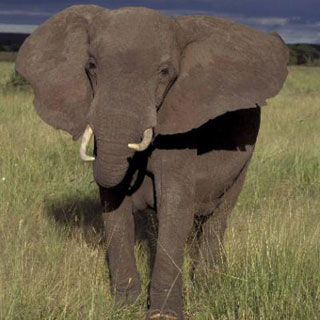
\includegraphics[width=0.8\linewidth]{elephant}
		\end{center}
		\blindtext[1]


\end{multicols}
% -----


%---
\section*{What a wonderful world}
This is such a wonderful document


\appendix

\section{Contact Information}
\subsection{Officers and Appointees}

\subsection{Note on Online Renewals}

\section{Membership Form}

%----
\end{document} 

